% Section content template for individual Educative lessons
% This file contains the actual content for a specific section
% Generated from Educative API section content

% Section: Class Diagram for LinkedIn
% Section ID: 5159026271977472
% Section Slug: class-diagram-for-linkedin
% Generated: 2025-12-14T13:35:12.968045

In this lesson, we'll identify and design classes, abstract classes, and interfaces based on the requirements gathered from the interviewer through our LinkedIn system.

\subsection{Components of LinkedIn}\label{YJktys6ljgDKx1_D4Zgl2}
\\
As mentioned, we will design the LinkedIn system using a bottom-up approach.

\subsubsection{Education, experience, and skill}\label{eP8RBNUEfReXjuWqN-nph}
\\
The \texttt{Education}, \texttt{Experience}, \texttt{Achievement}, and \texttt{Skill} classes provide relevant information and comprise the \texttt{Profile} class.
\\
These classes are represented below:

\begin{figure}[htbp]
 \centering
 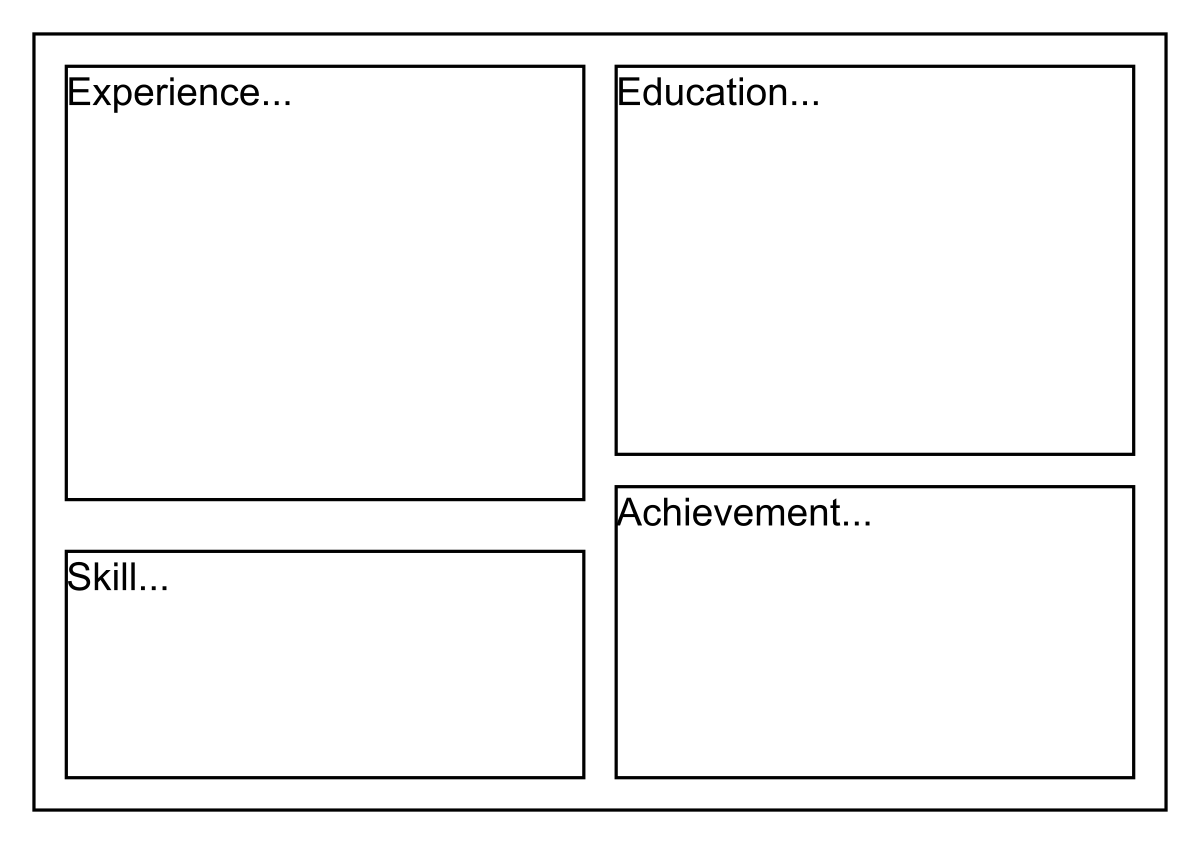
\includegraphics[width=0.5\textwidth]{Images/chapter_27/section_5159026271977472/4857855822659584.png}
 \caption{The Education, Achievement, Experience, and Skill classes}
\end{figure}

\textbf{R1:} Users should be able to add information to their profiles, including education, experiences, achievements, and skills.

\subsubsection{Recommendation, achievement, and analytics}\label{9Wd7DlQXt4gPSywBfWcnH}
\\
The \texttt{Recommendation}, and \texttt{Analytics} classes are used to provide relevant information and make up the \texttt{Profile} class.
\\
These classes are represented below:

\begin{figure}[htbp]
 \centering
 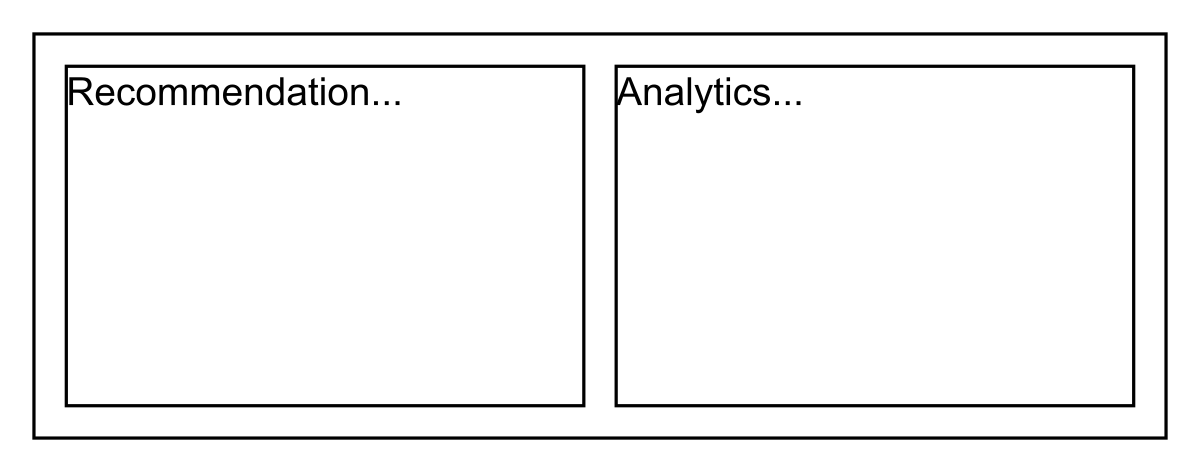
\includegraphics[width=0.5\textwidth]{Images/chapter_27/section_5159026271977472/5860396735791104.png}
 \caption{The Recommendation and Analytics classes}
\end{figure}

\textbf{R5:} Users should be able to view their number of connections, profile views, post impressions, and search appearances.
\\
\textbf{R6:} Users should be able to request and give recommendations to other users.

\subsubsection{Profile}\label{g8fdD7-Y9h32odtNFsNjX}
\\
The \texttt{Profile} class contains the personal information of a LinkedIn user, including their profile, cover photo, work experiences, educational details, skills, and achievements.
\\
The visual representation of the \texttt{Profile} class is given below:

\begin{figure}[htbp]
 \centering
 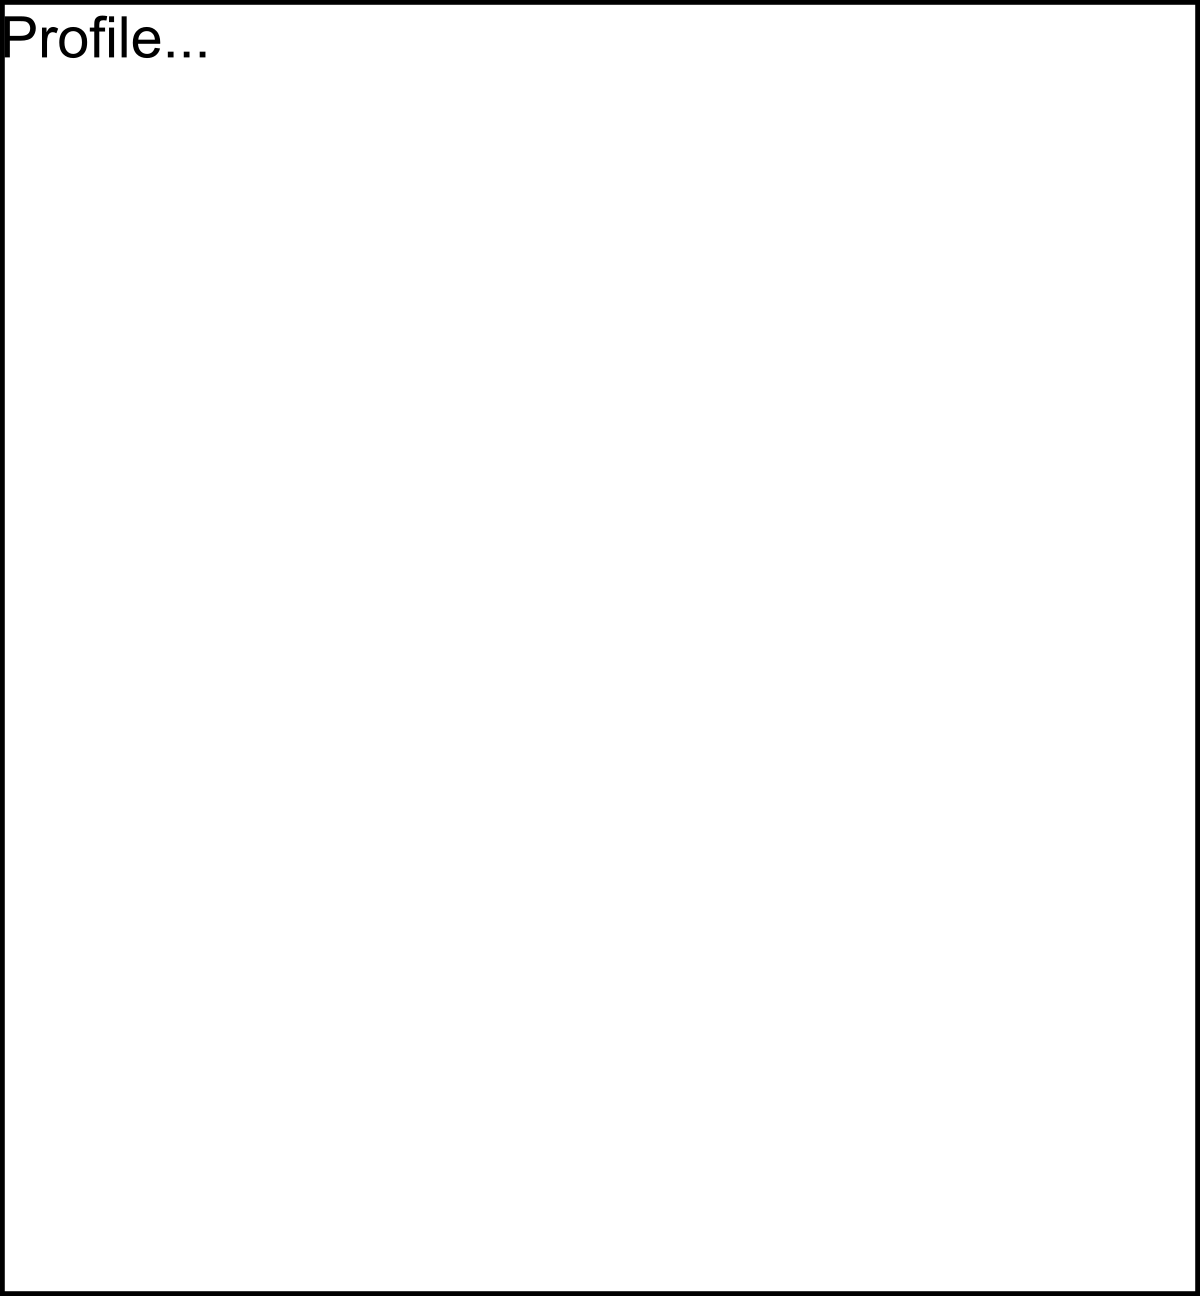
\includegraphics[width=0.5\textwidth]{Images/chapter_27/section_5159026271977472/6636942310768640.png}
 \caption{The Profile class}
\end{figure}

\textbf{R1:} Users should be able to add information to their profiles, including education, experiences, achievements, and skills.

\subsubsection{Company page, job, and group}\label{BfQjFmofUECvGiz2CeZc4}
\\
The \texttt{CompanyPage} class represents a particular page for a company that exists on LinkedIn. It contains the name, description, company size, and other relevant details.
\\
The \texttt{Job} class contains information about a job posting at a specific company, as well as current job openings.
\\
The \texttt{Group} class represents a particular group that exists on the LinkedIn platform. This will contain the name, description, total number of users, and a unique ID to identify the group.
\\
The representation of these classes is given below:

\begin{figure}[htbp]
 \centering
 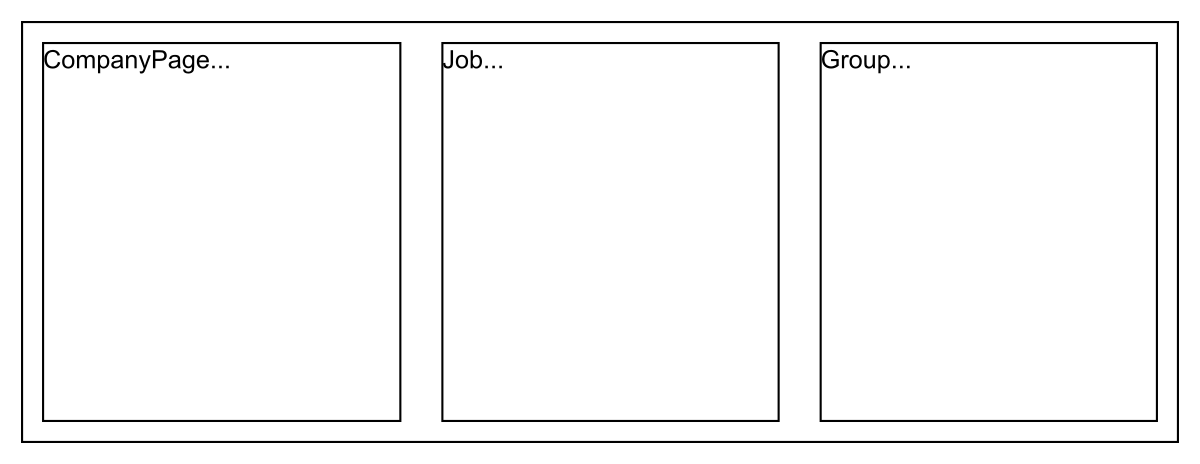
\includegraphics[width=0.5\textwidth]{Images/chapter_27/section_5159026271977472/4606841097945088.png}
 \caption{The CompanyPage, Job, and Group classes}
\end{figure}

\textbf{R11:} Users should be able to create company pages and follow other company pages.
\\
\textbf{R12:} Company pages should list job openings that users can apply for.
\\
\textbf{R13:} A user should be able to create and join groups.

\subsubsection{Post, comment, and message}\label{yIwfIxsMLJlu7gqq0RLrv}
\\
The \texttt{Post} class indicates a post made by a user. It contains information regarding its content, the number of reacts and shares of the post, and the owner of the post.
\\
The \texttt{Comment} class indicates a comment made by a user on a post. It includes information regarding its content, the number of reacts, and the owner of the comment.
\\
The \texttt{Message} class represents the message sent by a user to other users. Therefore, it contains content and multimedia elements, such as images or videos.
\\
The representation of the classes is shown below:

\begin{figure}[htbp]
 \centering
 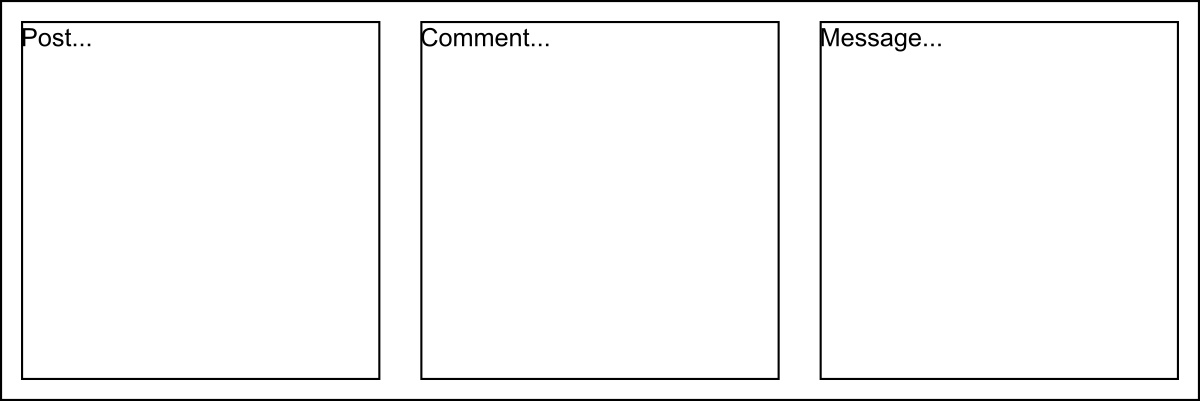
\includegraphics[width=0.5\textwidth]{Images/chapter_27/section_5159026271977472/5073768428077056.png}
 \caption{The Post, Comment, and Message classes}
\end{figure}

\textbf{R7:} Users should be able to write a new post.
\\
\textbf{R8:} Users should be able to react, share, and comment on a post and an existing comment.
\\
\textbf{R9:} A user should be able to send and receive messages from other users.

\subsubsection{Connection invitation}\label{SPF9kqCasGiY30Zs1wgYc}
\\
The \texttt{ConnectionInvitation} class describes the details of a connection invitation. It will contain the status of the connection invite and the methods that indicate whether the request was accepted or ignored.
\\
The class diagram of the \texttt{ConnectionInvitation} class is shown below:

\begin{figure}[htbp]
 \centering
 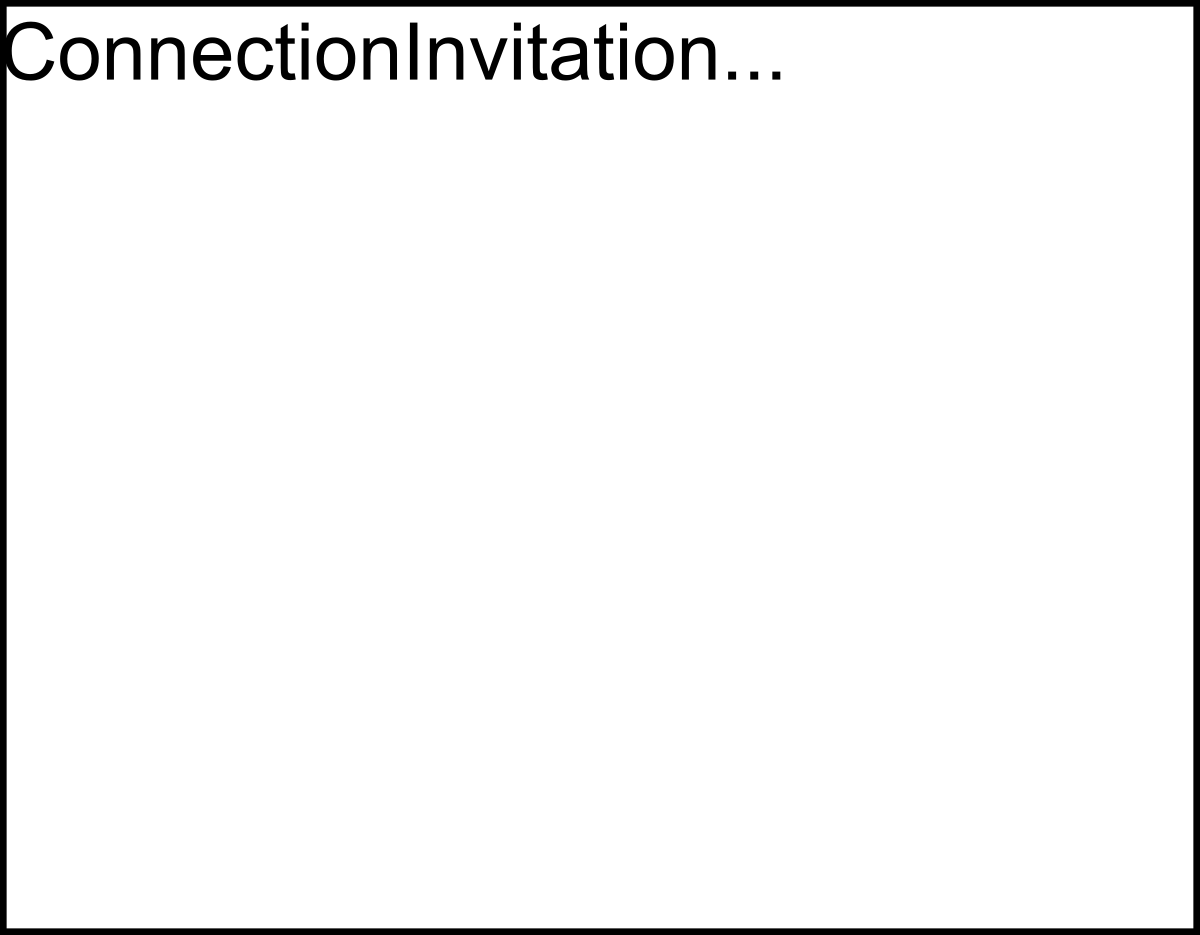
\includegraphics[width=0.5\textwidth]{Images/chapter_27/section_5159026271977472/6115389848420352.png}
 \caption{The ConnectionInvitation class}
\end{figure}

\textbf{R3:} Users should be able to send and cancel connection requests and respond to other users' connection requests by either accepting or ignoring them.

\subsubsection{Person}\label{uU1jV1DG3gJZ4BogMa01a}
\\
The \texttt{Person} is an abstract class that contains details like the name, address, and phone number. It is derived from the \texttt{User} class.
\\
\textbf{User}
\\
The \texttt{User} class is the main class of LinkedIn. It is responsible for various operations, such as applying for jobs, sending messages or friend requests to other users, creating posts and pages, joining groups, and numerous other tasks.
\\
These two classes are represented below:

\begin{figure}[htbp]
 \centering
 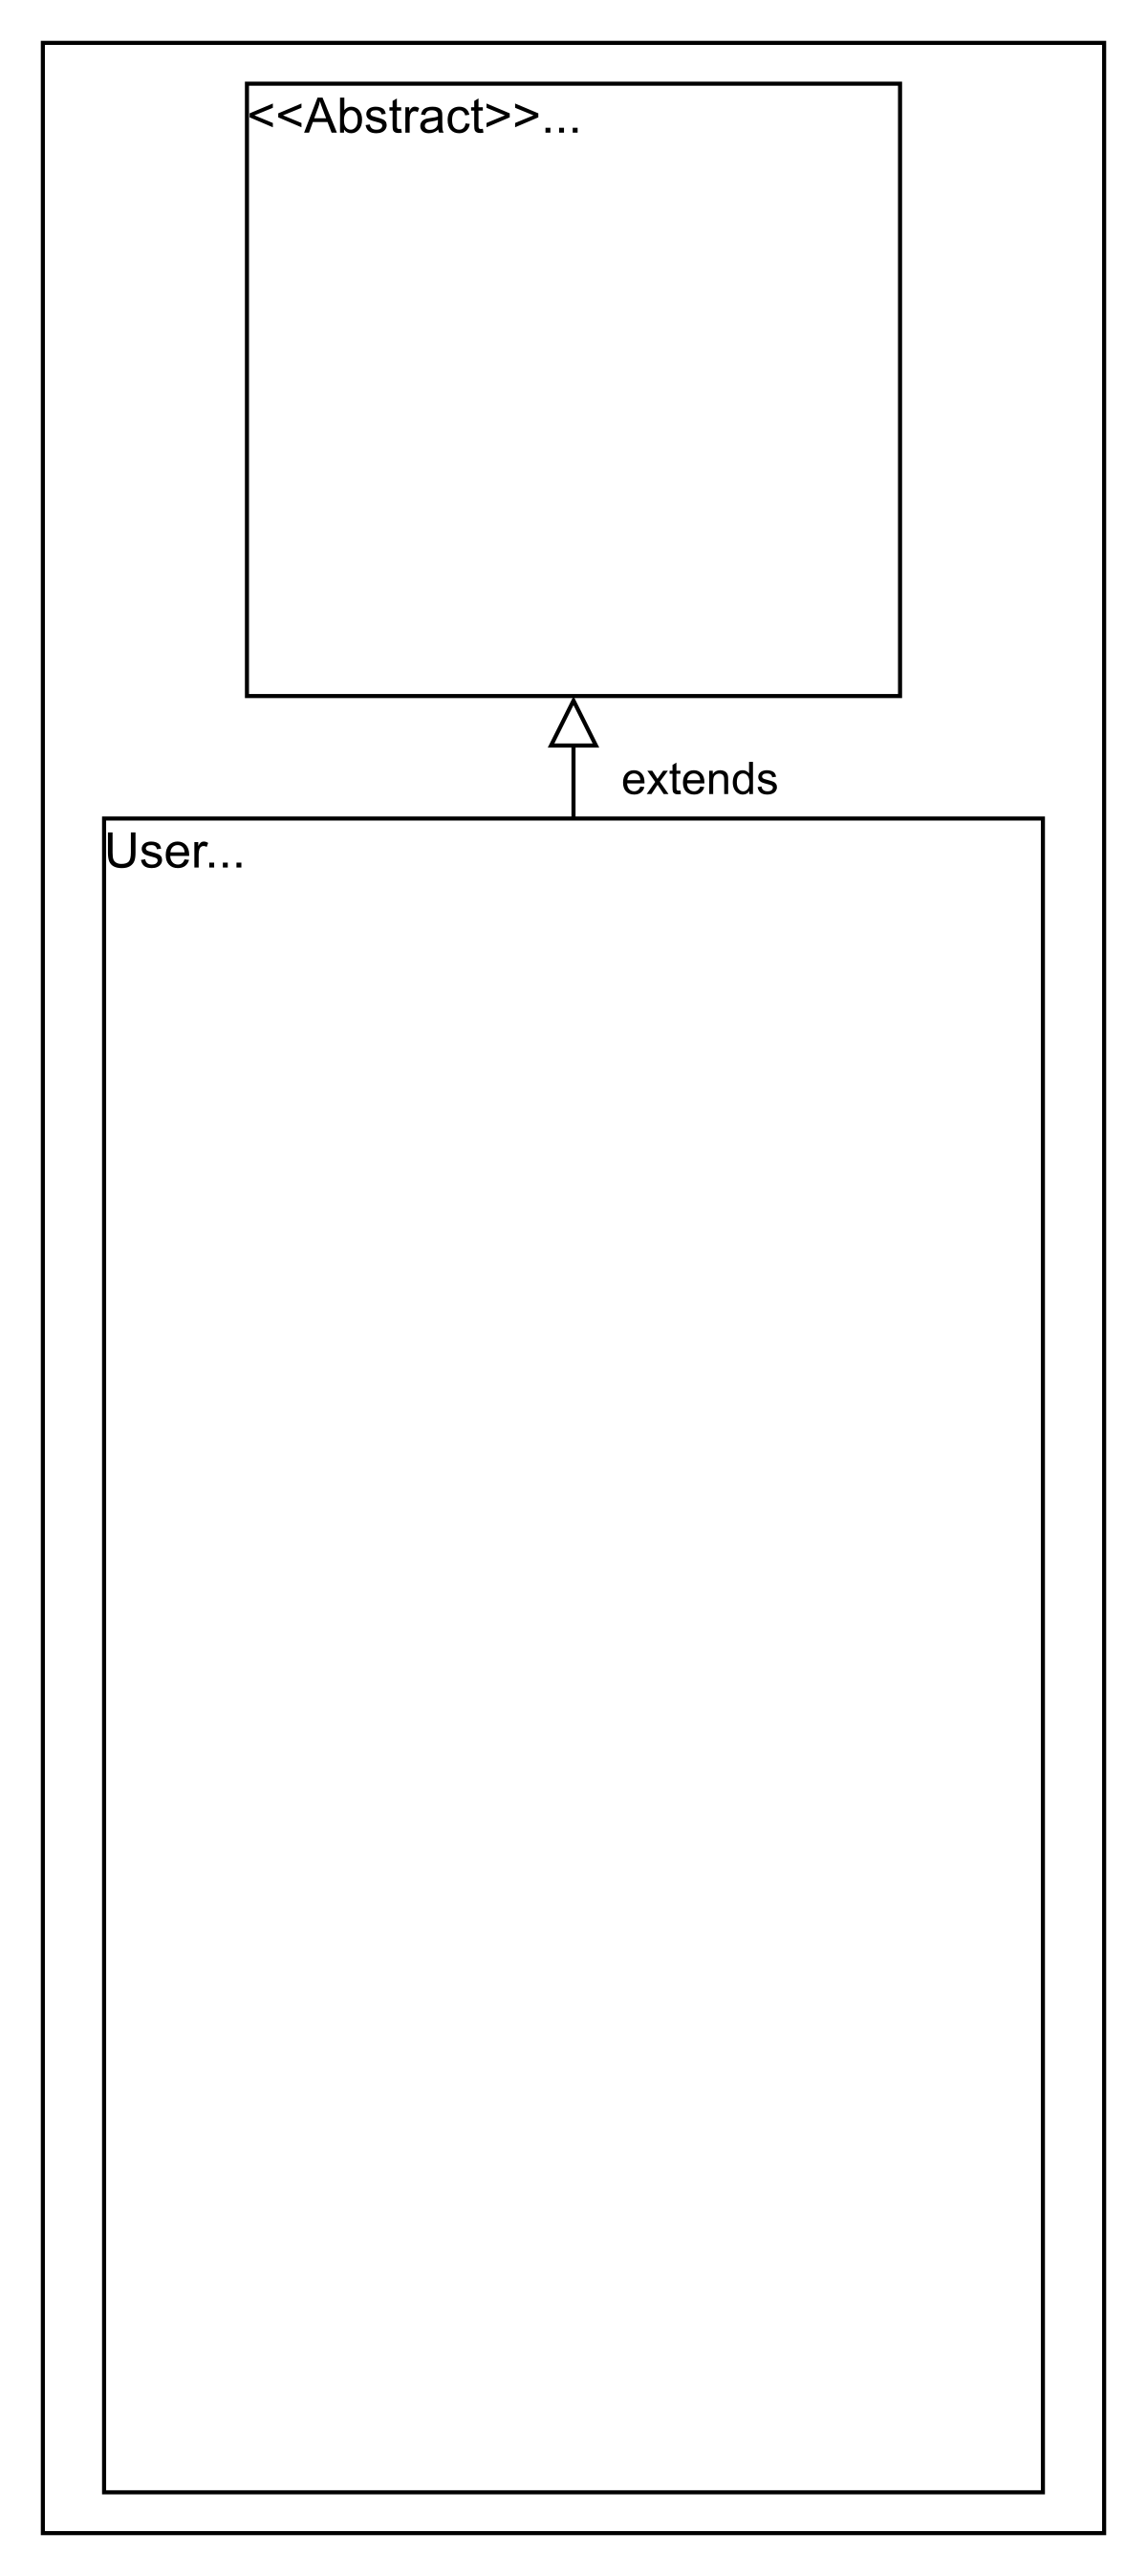
\includegraphics[width=0.5\textwidth]{Images/chapter_27/section_5159026271977472/5148041127264256.png}
 \caption{The Person and its derived classes}
\end{figure}

\subsubsection{Notification}\label{IrOM5UIERB-yBp8vIKGX6}
\\
The \texttt{Notification} class sends a notification using the built-in notification option. It is mainly responsible for sending notifications whenever any of the following conditions are met:

\begin{itemize}
\item
\protect\phantomsection\label{MvmpGHUoF0chZQg6NQnB4}
A connection invitation is received.
\item
\protect\phantomsection\label{A13ZimyFoRUmsadNtsdQ6}
A new message is received.
\item
\protect\phantomsection\label{oc2xsSiNLn34KztzXapz6}
A new comment is added to a post that a user has created or is following.
\item
\protect\phantomsection\label{6ZCnb7y0nkFW5OZ-YTmCk}
A new post has been created by a user or a company page that another user is following.
\item
\protect\phantomsection\label{XouLu2dVS8OpeIl-Eqr5a}
A user appeared in a search result.
\end{itemize}
\\
The UML representation of the class is shown below:

\begin{figure}[htbp]
 \centering
 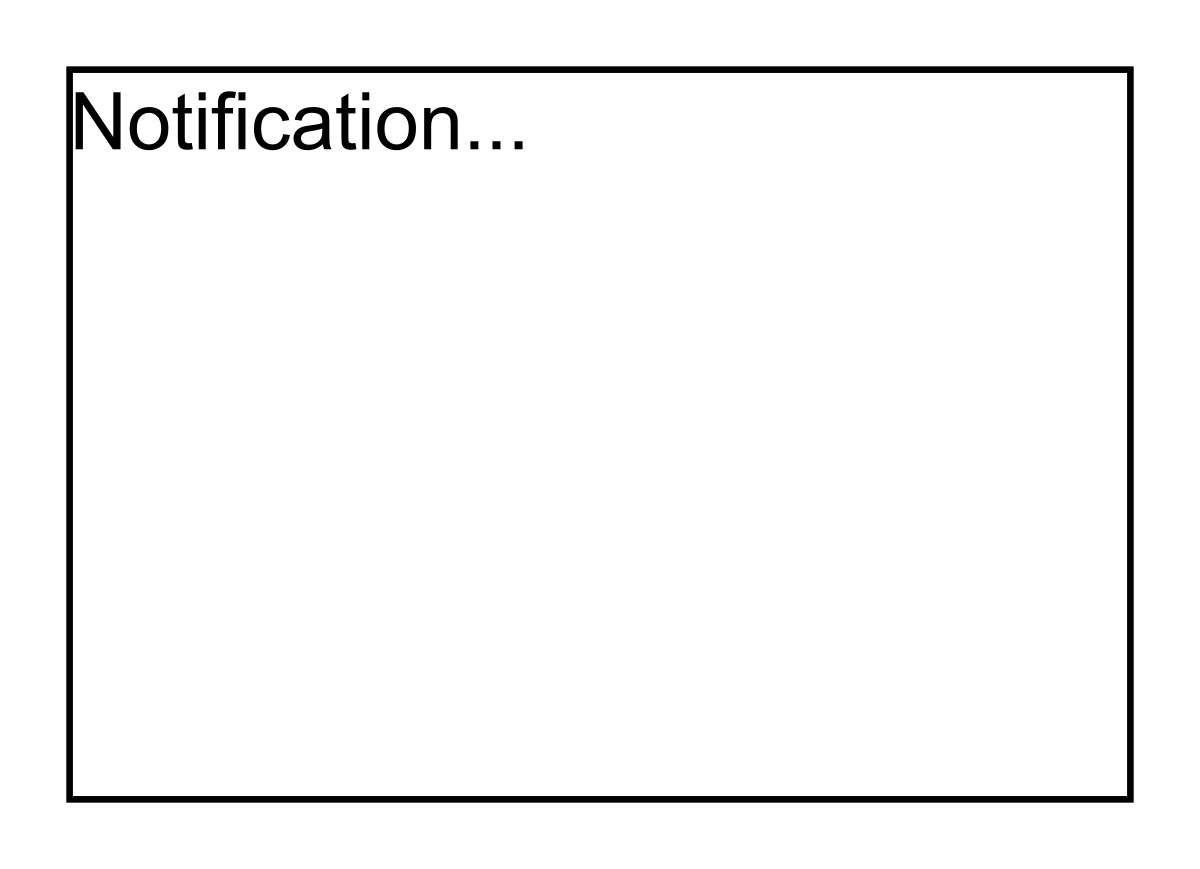
\includegraphics[width=0.5\textwidth]{Images/chapter_27/section_5159026271977472/6141182638686208.png}
 \caption{The Notification class}
\end{figure}

\textbf{R10:} The system should notify the user to inform them about messages, connection requests, search appearances, or comments on their post. or comments on their post.

\subsubsection{Search interface and search catalog}\label{44LcGxSoy8F1-kiv8oGN_}
\\
The \texttt{Search} class enables users to search for specific users, companies, groups, or job openings. It also returns the list of respective components.
\\
The representation of the \texttt{Search} class is given below:

\begin{figure}[htbp]
 \centering
 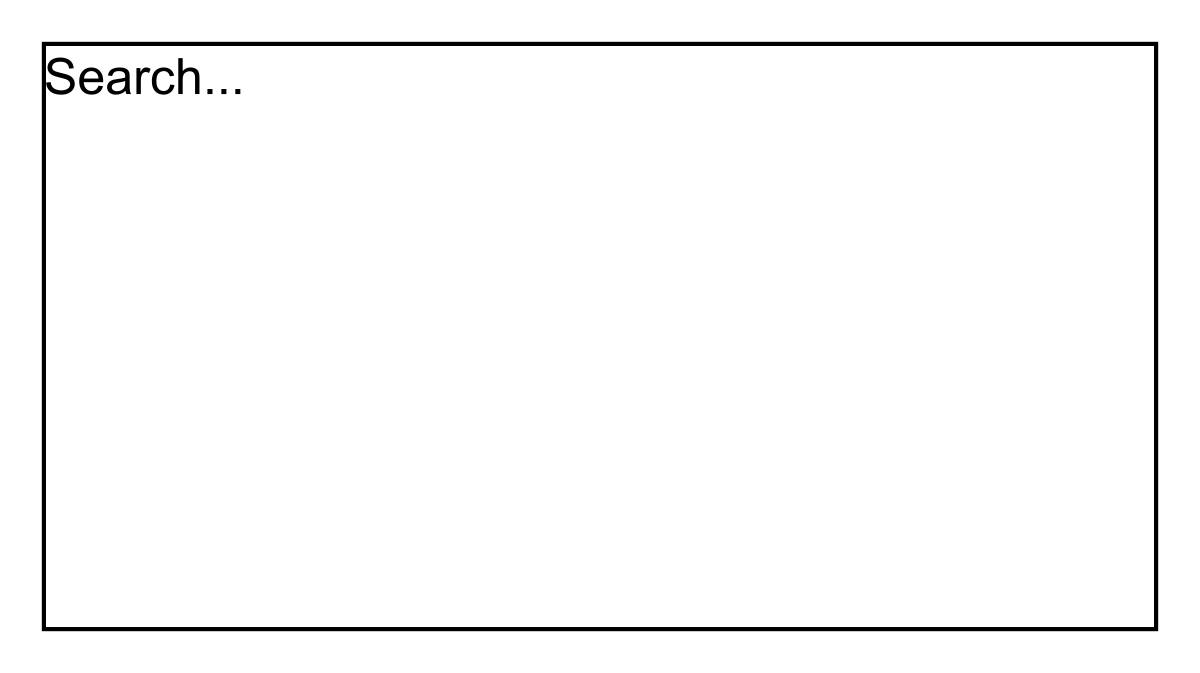
\includegraphics[width=0.5\textwidth]{Images/chapter_27/section_5159026271977472/4743565400735744.png}
 \caption{The SearchCatalog class and the Search interface}
\end{figure}

\textbf{R2:} Users should be able to search for and view pages, groups, and other users.

\subsubsection{Enumerations}\label{oBZXQaMYGjx34tfS1i-2u}
\\
The enumerations required in the LinkedIn design are provided below:

\begin{itemize}
\item
\protect\phantomsection\label{1kAWTV7Efduf6tLHCNCIu}
\texttt{ConnectionInviteStatus}: The connection invite status describes the status of a connection invitation---whether it is pending, accepted, or ignored.
\item
\protect\phantomsection\label{xRpQ4Kvl1fMI5-44I7H-H}
\texttt{JobStatus}: The job status describes the current status of a job posting---whether it is open, on hold, or closed.
\end{itemize}

\begin{figure}[htbp]
 \centering
 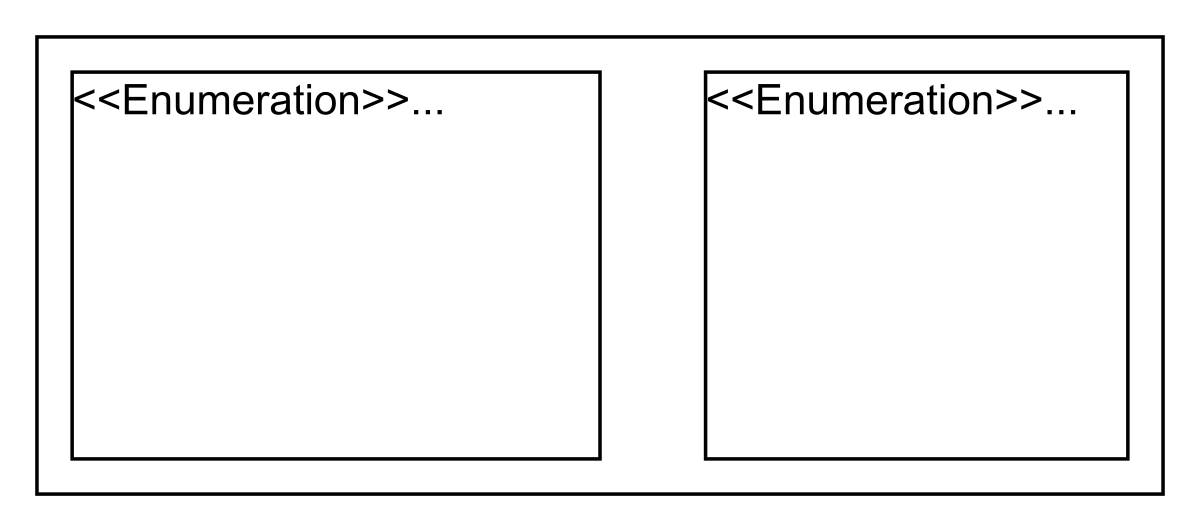
\includegraphics[width=0.5\textwidth]{Images/chapter_27/section_5159026271977472/4928474597687296.png}
 \caption{Enums in LinkedIn}
\end{figure}

\subsubsection{Custom data type}\label{t5g-1ILeHSC7c6cMdUIa_}
\\
We need to create a custom data type, \texttt{Address}, which stores the location of a LinkedIn user.

\begin{figure}[htbp]
 \centering
 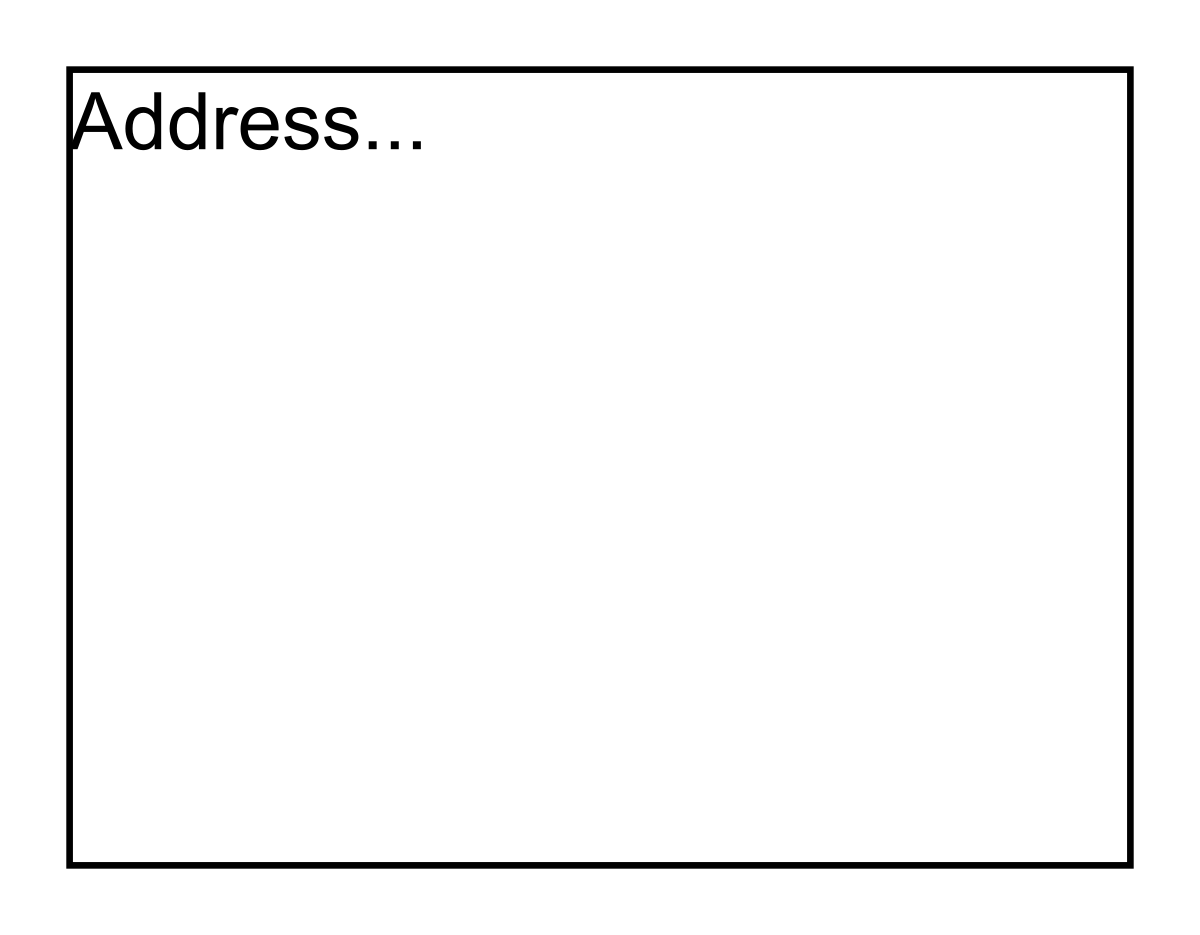
\includegraphics[width=0.5\textwidth]{Images/chapter_27/section_5159026271977472/6641278077763584.png}
 \caption{The Address custom data type}
\end{figure}

\subsection{Relationship between the classes}\label{8ZgjUudfjSA78wa1AzCq-}
\\
Now, we'll discuss the relationships between the classes we have defined above in our LinkedIn system.

\subsubsection{Association}\label{WKVjOFgc7TE3tgM8FcZI_}
\\
The class diagram has the following association relationships:

\begin{itemize}
\item
\protect\phantomsection\label{HxNk5Hcyz4IS2t0m_bzD6}
The \texttt{User} class has a one-way association with the following:

\begin{itemize}
\item
Itself
\item
The \texttt{CompanyPage}, \texttt{Group}, \texttt{Job}, \texttt{Post}, \texttt{Comment}, \texttt{Message}, and \texttt{ConnectionInvitation} classes
\item
The \texttt{Search} class
\end{itemize}
\item
\protect\phantomsection\label{jZqsL0CaIj-yRc9EkvHSt}
The \texttt{Notification} class has a one-way association with the \texttt{Message}, \texttt{Post}, \texttt{Comment}, \texttt{ConnectionInvitation}, \texttt{search}, and \texttt{Recommendation} classes.
\end{itemize}

\begin{figure}[htbp]
 \centering
 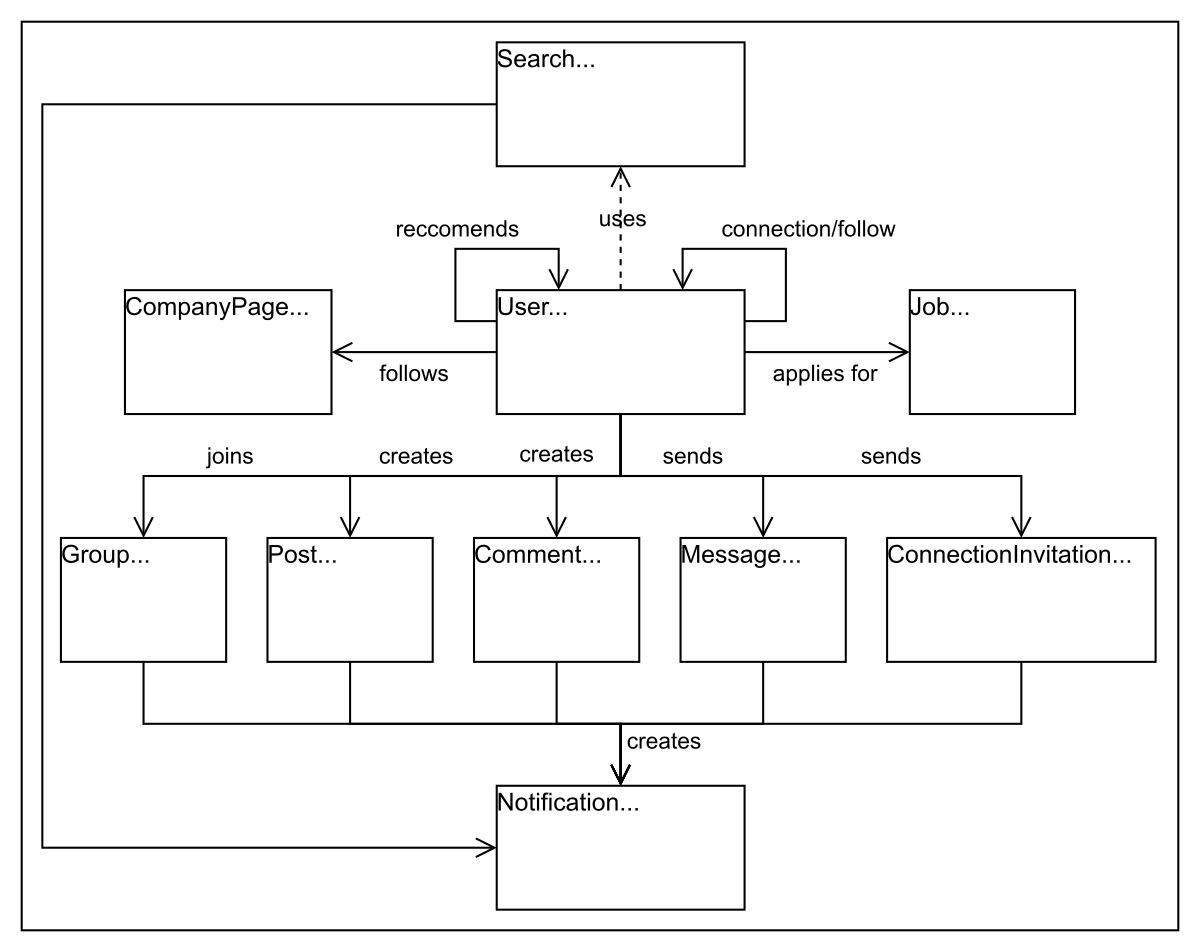
\includegraphics[width=0.5\textwidth]{Images/chapter_27/section_5159026271977472/5361411042443264.png}
 \caption{The association relationship between classes}
\end{figure}

\subsubsection{Composition}\label{u0MEHZwU89pS3bbyxQ3vI}
\\
The class diagram has the following composition relationships:

\begin{itemize}
\item
\protect\phantomsection\label{qF0Bhzatk2LOqv7MJTx4U}
The \texttt{Person} class is composed of the \texttt{Account} class.
\item
\protect\phantomsection\label{P_40iI-hXF4tdrmwyXBUu}
The \texttt{User} class is composed of the \texttt{Profile} class.
\item
\protect\phantomsection\label{GA9xT4kZEosV9vK77MZvO}
The \texttt{Profile} class comprises the \texttt{Experience}, \texttt{Education}, \texttt{Skill}, \texttt{Achievement}, \texttt{Recommendation}, and \texttt{Analytics} classes.
\item
\protect\phantomsection\label{NMPbl6bocQZZeMc_EcJCT}
The \texttt{Post} class is composed of the \texttt{Comment} class.
\item
\protect\phantomsection\label{16K2tSLJSICR2sMDvDl4s}
The \texttt{CompanyPage} class is composed of the \texttt{Job} class.
\end{itemize}

\begin{figure}[htbp]
 \centering
 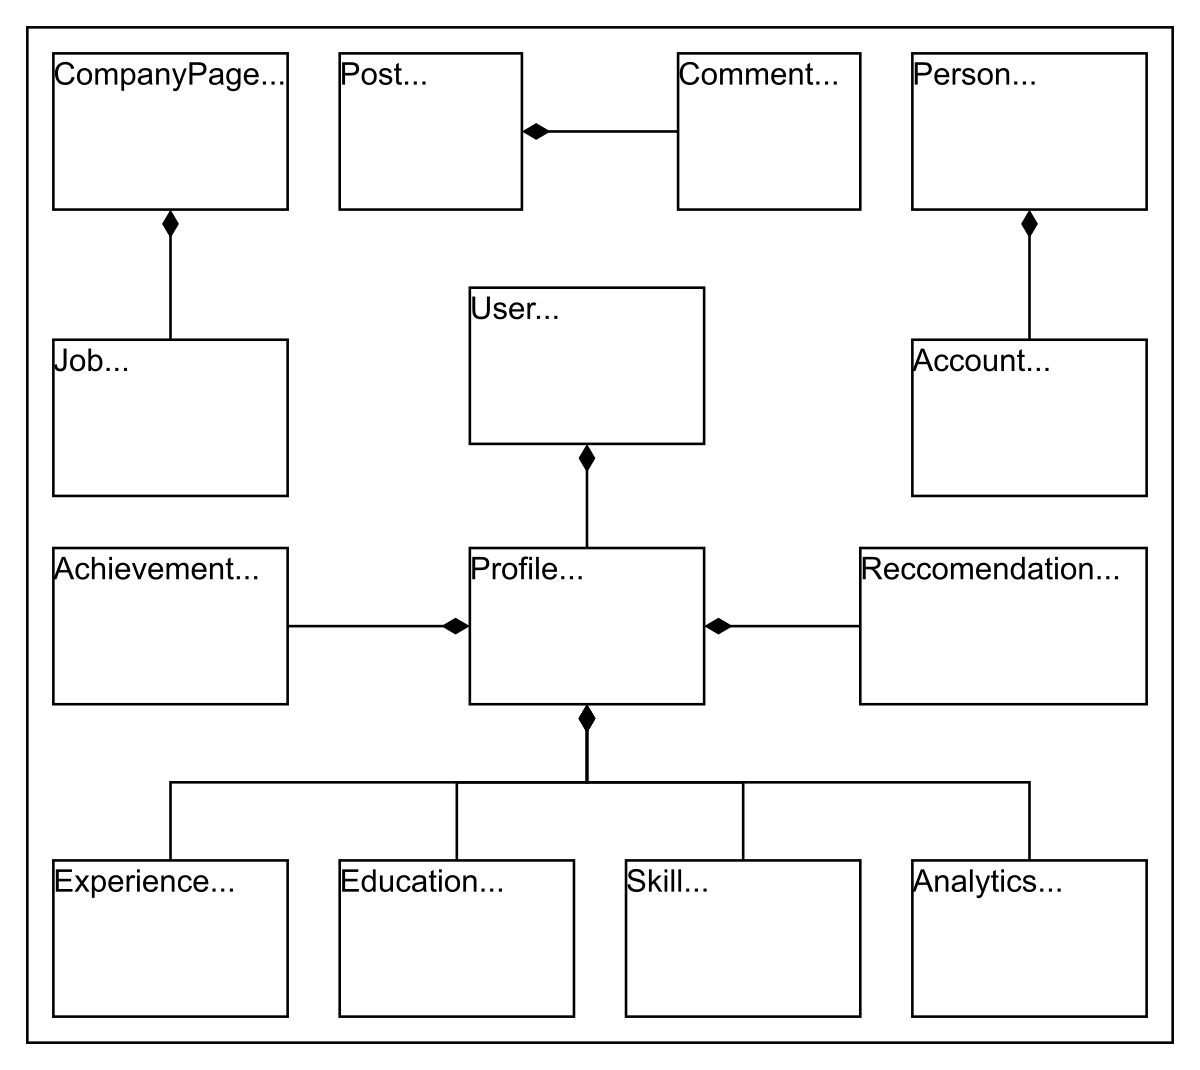
\includegraphics[width=0.5\textwidth]{Images/chapter_27/section_5159026271977472/5191715374628864.png}
 \caption{The composition relationship between classes}
\end{figure}

\subsubsection{Inheritance}\label{aGkOU5GolUuv_olsHlVBE}
\\
The following classes demonstrate an inheritance relationship:

\begin{itemize}
\item
\protect\phantomsection\label{zGO9iP4XQ5R0j7PM84lSC}
The \texttt{User} classes extend the \texttt{Person} class.
\end{itemize}
\begin{quote}
\textbf{Note:} We have already discussed the inheritance relationship between classes in the component section above one by one.
\end{quote}
\subsection{Class diagram of LinkedIn}\label{1pEKtLyCJGMV5-M0gjATg}
\\
In this section, we outline the multiplicity (cardinality) relationships between the main classes in our~LinkedIn design system. For each relationship, we explain the allowed number of instances on each side and the real-world or design rationale behind the connection. Understanding these relationships is crucial for modeling how different entities interact and collaborate to support key workflows within the system.

\begin{center}
{\def\LTcaptype{none} % do not increment counter
\begin{longtable}[]{@{}
>{\raggedright\arraybackslash} p{(\linewidth - 6\tabcolsep) * \real{0.2500}}
>{\raggedright\arraybackslash} p{(\linewidth - 6\tabcolsep) * \real{0.2500}}
>{\raggedright\arraybackslash} p{(\linewidth - 6\tabcolsep) * \real{0.2500}}
>{\raggedright\arraybackslash} p{(\linewidth - 6\tabcolsep) * \real{0.2500}}@{}}
\toprule\noalign{}
\endhead
\bottomrule\noalign{}
\endlastfoot
\begin{minipage}[t]{\linewidth}\raggedright
\textbf{Source}
\end{minipage} & \begin{minipage}[t]{\linewidth}\raggedright
\textbf{Target}
\end{minipage} & \begin{minipage}[t]{\linewidth}\raggedright
\textbf{Multiplicity}
\end{minipage} & \begin{minipage}[t]{\linewidth}\raggedright
\textbf{Explanation}
\end{minipage} \\
\begin{minipage}[t]{\linewidth}\raggedright
Person
\end{minipage} & \begin{minipage}[t]{\linewidth}\raggedright
User
\end{minipage} & \begin{minipage}[t]{\linewidth}\raggedright
1 -- 1
\end{minipage} & \begin{minipage}[t]{\linewidth}\raggedright
User extends Person
\end{minipage} \\
\begin{minipage}[t]{\linewidth}\raggedright
User
\end{minipage} & \begin{minipage}[t]{\linewidth}\raggedright
Profile
\end{minipage} & \begin{minipage}[t]{\linewidth}\raggedright
1 -- 1
\end{minipage} & \begin{minipage}[t]{\linewidth}\raggedright
Each user has exactly one profile
\end{minipage} \\
\begin{minipage}[t]{\linewidth}\raggedright
User
\end{minipage} & \begin{minipage}[t]{\linewidth}\raggedright
CompanyPage
\end{minipage} & \begin{minipage}[t]{\linewidth}\raggedright
1 -- 0..*
\end{minipage} & \begin{minipage}[t]{\linewidth}\raggedright
A user can create multiple company pages
\end{minipage} \\
\begin{minipage}[t]{\linewidth}\raggedright
User
\end{minipage} & \begin{minipage}[t]{\linewidth}\raggedright
User
\end{minipage} & \begin{minipage}[t]{\linewidth}\raggedright
0..* -- 0..*
\end{minipage} & \begin{minipage}[t]{\linewidth}\raggedright
Users can follow or connect with many other users
\end{minipage} \\
\begin{minipage}[t]{\linewidth}\raggedright
User
\end{minipage} & \begin{minipage}[t]{\linewidth}\raggedright
Group
\end{minipage} & \begin{minipage}[t]{\linewidth}\raggedright
1 -- 0..*
\end{minipage} & \begin{minipage}[t]{\linewidth}\raggedright
A user can join or create multiple groups
\end{minipage} \\
\begin{minipage}[t]{\linewidth}\raggedright
User
\end{minipage} & \begin{minipage}[t]{\linewidth}\raggedright
Comment
\end{minipage} & \begin{minipage}[t]{\linewidth}\raggedright
1 -- 0..*
\end{minipage} & \begin{minipage}[t]{\linewidth}\raggedright
A user can make multiple comments
\end{minipage} \\
\begin{minipage}[t]{\linewidth}\raggedright
User
\end{minipage} & \begin{minipage}[t]{\linewidth}\raggedright
Message
\end{minipage} & \begin{minipage}[t]{\linewidth}\raggedright
1 -- 0..*
\end{minipage} & \begin{minipage}[t]{\linewidth}\raggedright
A user can send or receive multiple messages
\end{minipage} \\
\begin{minipage}[t]{\linewidth}\raggedright
User
\end{minipage} & \begin{minipage}[t]{\linewidth}\raggedright
Post
\end{minipage} & \begin{minipage}[t]{\linewidth}\raggedright
1 -- 0..*
\end{minipage} & \begin{minipage}[t]{\linewidth}\raggedright
A user can create multiple posts
\end{minipage} \\
\begin{minipage}[t]{\linewidth}\raggedright
User
\end{minipage} & \begin{minipage}[t]{\linewidth}\raggedright
Job
\end{minipage} & \begin{minipage}[t]{\linewidth}\raggedright
1 -- 0..*
\end{minipage} & \begin{minipage}[t]{\linewidth}\raggedright
A user can apply to multiple jobs
\end{minipage} \\
\begin{minipage}[t]{\linewidth}\raggedright
User
\end{minipage} & \begin{minipage}[t]{\linewidth}\raggedright
ConnectionInvitation
\end{minipage} & \begin{minipage}[t]{\linewidth}\raggedright
1 -- 0..*
\end{minipage} & \begin{minipage}[t]{\linewidth}\raggedright
A user can send or receive multiple connection invitations
\end{minipage} \\
\begin{minipage}[t]{\linewidth}\raggedright
Profile
\end{minipage} & \begin{minipage}[t]{\linewidth}\raggedright
Analytics
\end{minipage} & \begin{minipage}[t]{\linewidth}\raggedright
1 -- 1
\end{minipage} & \begin{minipage}[t]{\linewidth}\raggedright
A profile has one set of analytics data
\end{minipage} \\
\begin{minipage}[t]{\linewidth}\raggedright
Profile
\end{minipage} & \begin{minipage}[t]{\linewidth}\raggedright
Experience
\end{minipage} & \begin{minipage}[t]{\linewidth}\raggedright
1 -- 0..*
\end{minipage} & \begin{minipage}[t]{\linewidth}\raggedright
A profile can include multiple experiences
\end{minipage} \\
\begin{minipage}[t]{\linewidth}\raggedright
Profile
\end{minipage} & \begin{minipage}[t]{\linewidth}\raggedright
Education
\end{minipage} & \begin{minipage}[t]{\linewidth}\raggedright
1 -- 0..*
\end{minipage} & \begin{minipage}[t]{\linewidth}\raggedright
A profile can include multiple education entries
\end{minipage} \\
\begin{minipage}[t]{\linewidth}\raggedright
Profile
\end{minipage} & \begin{minipage}[t]{\linewidth}\raggedright
Skill
\end{minipage} & \begin{minipage}[t]{\linewidth}\raggedright
0..* -- 0..*
\end{minipage} & \begin{minipage}[t]{\linewidth}\raggedright
A profile can list multiple skills
\end{minipage} \\
\begin{minipage}[t]{\linewidth}\raggedright
Profile
\end{minipage} & \begin{minipage}[t]{\linewidth}\raggedright
Achievement
\end{minipage} & \begin{minipage}[t]{\linewidth}\raggedright
1 -- 0..*
\end{minipage} & \begin{minipage}[t]{\linewidth}\raggedright
A profile can include multiple achievements
\end{minipage} \\
\begin{minipage}[t]{\linewidth}\raggedright
Profile
\end{minipage} & \begin{minipage}[t]{\linewidth}\raggedright
Recommendation
\end{minipage} & \begin{minipage}[t]{\linewidth}\raggedright
1 -- 0..*
\end{minipage} & \begin{minipage}[t]{\linewidth}\raggedright
A profile can contain multiple recommendations
\end{minipage} \\
\begin{minipage}[t]{\linewidth}\raggedright
CompanyPage
\end{minipage} & \begin{minipage}[t]{\linewidth}\raggedright
Job
\end{minipage} & \begin{minipage}[t]{\linewidth}\raggedright
1 -- 0..*
\end{minipage} & \begin{minipage}[t]{\linewidth}\raggedright
A company page can list multiple jobs
\end{minipage} \\
\begin{minipage}[t]{\linewidth}\raggedright
Job
\end{minipage} & \begin{minipage}[t]{\linewidth}\raggedright
User
\end{minipage} & \begin{minipage}[t]{\linewidth}\raggedright
1 -- 1
\end{minipage} & \begin{minipage}[t]{\linewidth}\raggedright
One user posts a job
\end{minipage} \\
\begin{minipage}[t]{\linewidth}\raggedright
Job
\end{minipage} & \begin{minipage}[t]{\linewidth}\raggedright
Address
\end{minipage} & \begin{minipage}[t]{\linewidth}\raggedright
1 -- 1
\end{minipage} & \begin{minipage}[t]{\linewidth}\raggedright
A job has one location
\end{minipage} \\
\begin{minipage}[t]{\linewidth}\raggedright
Job
\end{minipage} & \begin{minipage}[t]{\linewidth}\raggedright
CompanyPage
\end{minipage} & \begin{minipage}[t]{\linewidth}\raggedright
1 -- 1
\end{minipage} & \begin{minipage}[t]{\linewidth}\raggedright
A job belongs to one company page
\end{minipage} \\
\begin{minipage}[t]{\linewidth}\raggedright
Comment
\end{minipage} & \begin{minipage}[t]{\linewidth}\raggedright
Post
\end{minipage} & \begin{minipage}[t]{\linewidth}\raggedright
0..* -- 1
\end{minipage} & \begin{minipage}[t]{\linewidth}\raggedright
A post can have multiple comments
\end{minipage} \\
\begin{minipage}[t]{\linewidth}\raggedright
Comment
\end{minipage} & \begin{minipage}[t]{\linewidth}\raggedright
User
\end{minipage} & \begin{minipage}[t]{\linewidth}\raggedright
1 -- 1
\end{minipage} & \begin{minipage}[t]{\linewidth}\raggedright
One user writes each comment
\end{minipage} \\
\begin{minipage}[t]{\linewidth}\raggedright
Post
\end{minipage} & \begin{minipage}[t]{\linewidth}\raggedright
Comment
\end{minipage} & \begin{minipage}[t]{\linewidth}\raggedright
1 -- 0..*
\end{minipage} & \begin{minipage}[t]{\linewidth}\raggedright
A post can have multiple comments
\end{minipage} \\
\begin{minipage}[t]{\linewidth}\raggedright
Message
\end{minipage} & \begin{minipage}[t]{\linewidth}\raggedright
User
\end{minipage} & \begin{minipage}[t]{\linewidth}\raggedright
1 -- 0..*
\end{minipage} & \begin{minipage}[t]{\linewidth}\raggedright
A message can have one sender and multiple recipients
\end{minipage} \\
\begin{minipage}[t]{\linewidth}\raggedright
Group
\end{minipage} & \begin{minipage}[t]{\linewidth}\raggedright
User
\end{minipage} & \begin{minipage}[t]{\linewidth}\raggedright
1 -- 0..*
\end{minipage} & \begin{minipage}[t]{\linewidth}\raggedright
A group can have many members (users)
\end{minipage} \\
\begin{minipage}[t]{\linewidth}\raggedright
ConnectionInvitation
\end{minipage} & \begin{minipage}[t]{\linewidth}\raggedright
User
\end{minipage} & \begin{minipage}[t]{\linewidth}\raggedright
1 -- 1
\end{minipage} & \begin{minipage}[t]{\linewidth}\raggedright
An invitation is between exactly two users
\end{minipage} \\
\begin{minipage}[t]{\linewidth}\raggedright
Notification
\end{minipage} & \begin{minipage}[t]{\linewidth}\raggedright
User
\end{minipage} & \begin{minipage}[t]{\linewidth}\raggedright
1 -- 1
\end{minipage} & \begin{minipage}[t]{\linewidth}\raggedright
Each notification is sent to one user
\end{minipage} \\
\begin{minipage}[t]{\linewidth}\raggedright
Search
\end{minipage} & \begin{minipage}[t]{\linewidth}\raggedright
User / CompanyPage / Job / Group
\end{minipage} & \begin{minipage}[t]{\linewidth}\raggedright
1 -- 0..*
\end{minipage} & \begin{minipage}[t]{\linewidth}\raggedright
A search can include users, companies, jobs, or groups
\end{minipage} \\
\end{longtable}
}
\end{center}

Here's the complete class diagram for LinkedIn:

\begin{figure}[htbp]
 \centering
 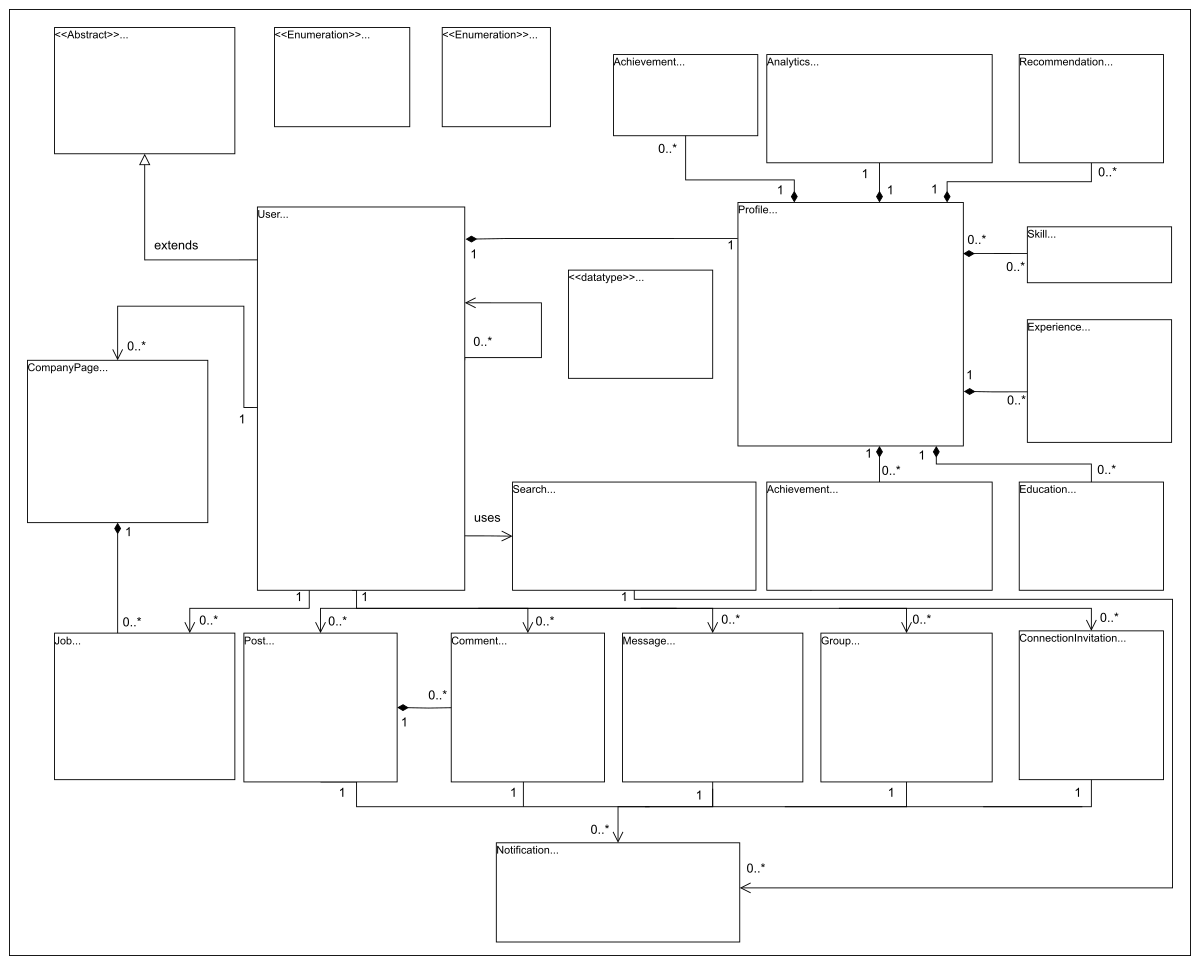
\includegraphics[width=0.5\textwidth]{Images/chapter_27/section_5159026271977472/4582804888092672.png}
 \caption{The class diagram of LinkedIn}
\end{figure}

\subsection{Design pattern}\label{1OeGJ3qZqw26eXvNW1DLf}
\\
The following design patterns have been used in the class diagram:

\begin{itemize}
\item
We know that users can create various types of objects, such as connection invitations, posts, comments, and job listings. To centralize and manage the creation of these objects, we can use theFactory design pattern.
\item
We understand that users need to be notified when specific actions occur, such as receiving a connection request, appearing in a search result, or receiving a comment on a post. To handle this automatic notification mechanism, we can use the Observer design pattern.
\item
We recognize that certain services, such as search and notification, should utilize a single, shared instance across the entire system. To enforce that only one instance of such a service exists, we can use the Singleton design pattern.
\item
We know that users can search for various entities, such as users, jobs, companies, or groups, and the search logic may differ for each. To encapsulate these different search behaviors and allow them to be swapped easily, we can use the Strategy design pattern.
\item
We know that a post or comment might need additional behaviors such as adding reactions, sharing, or threading replies. To extend these features without altering the base class, we can use the Decorator design pattern.
\end{itemize}

\subsection{AI-powered trainer}\label{RxKBY7ueP2O1EhlQHu9JL}
\\
At this stage, everything should be clear. If you encounter any confusion or ambiguity, feel free to utilize the interactive AI-enabled widget below to seek clarification. This tool is designed to help you strengthen your understanding of the concepts.

\begin{figure}[htbp]
 \centering
 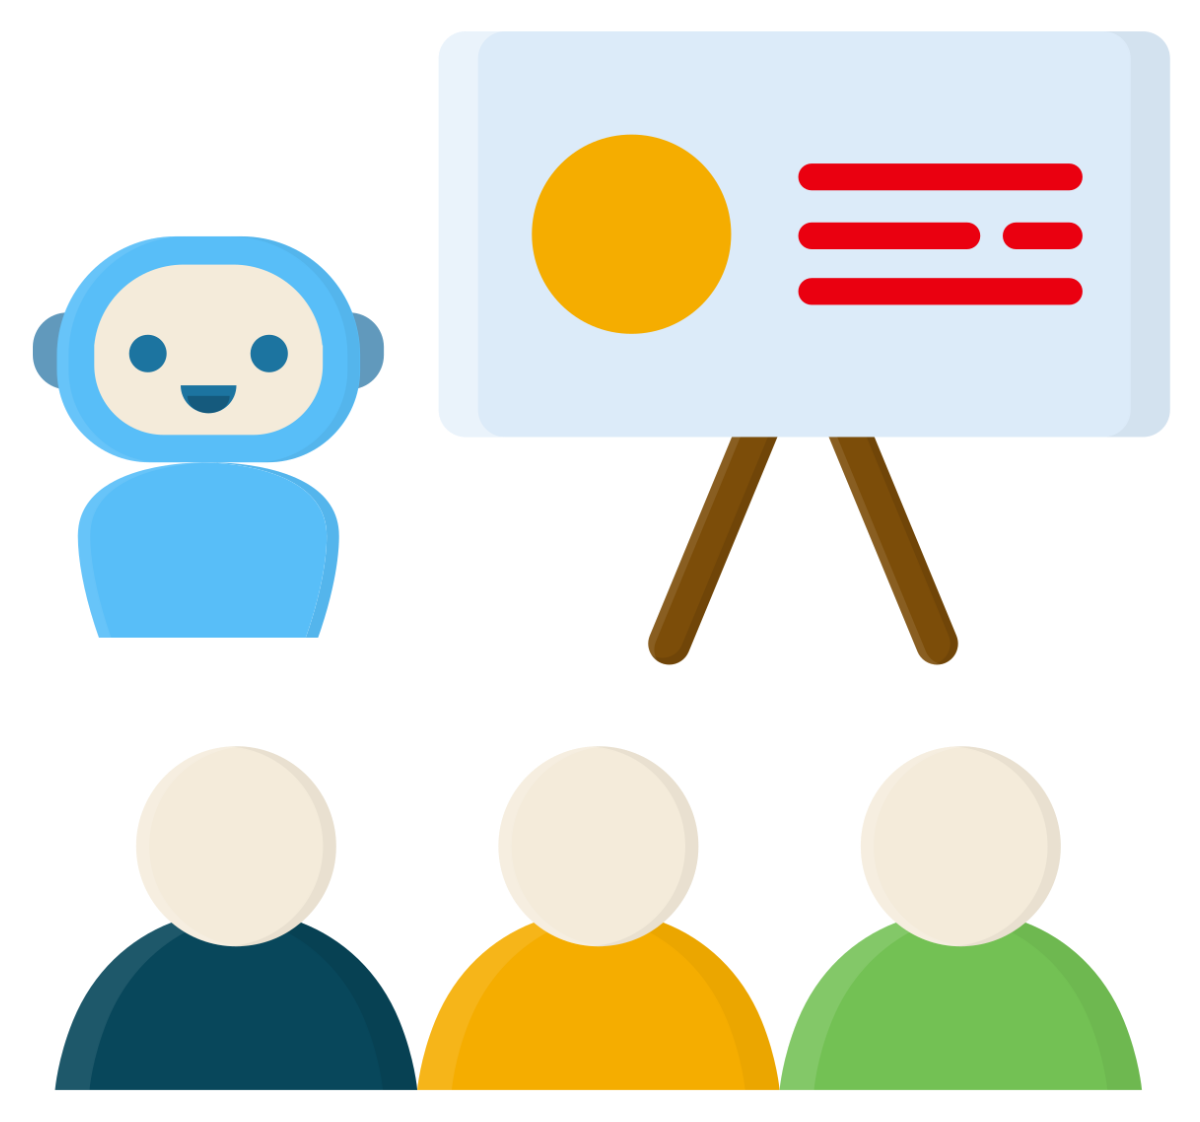
\includegraphics[width=0.15\textwidth]{Images/chapter_27/section_5159026271977472/4795644341256192.png}
 
\end{figure}

We have completed the class diagram of LinkedIn according to the requirements. Now, let's design the sequence diagram of LinkedIn in the next lesson.

% End of section content